\documentclass[border=10pt]{standalone}

\usepackage{tikz}
\usetikzlibrary{decorations.markings,calc,arrows}

% Load style for signal-flow graphs
%%%
%%% For the SFGs
%%%
\tikzset{%
	% Style of the node
	Node/.style={circle,thick,draw=black,inner sep=0, minimum size=0.15cm},
	% Style of the node label
	NodeName/.style={font=\footnotesize,black,outer sep=1},
	% Style of the branche label
	ArrowName/.style={font=\footnotesize,auto,outer sep=1},
	% Style of the branch
	Connection/.style={thick},
	->-/.style={decoration={
			markings,
			mark=at position #1 with {\draw[->,>=latex',line width=2pt](0pt,0)--(4pt,0);}},
		postaction={decorate}},
	->-/.default=0.50,
	MarkMiddle/.style={decoration={
			markings,
			mark=at position 0.5 with {\node[NodeName](middle_#1){};}},
		postaction={decorate}},
}

\begin{document}
	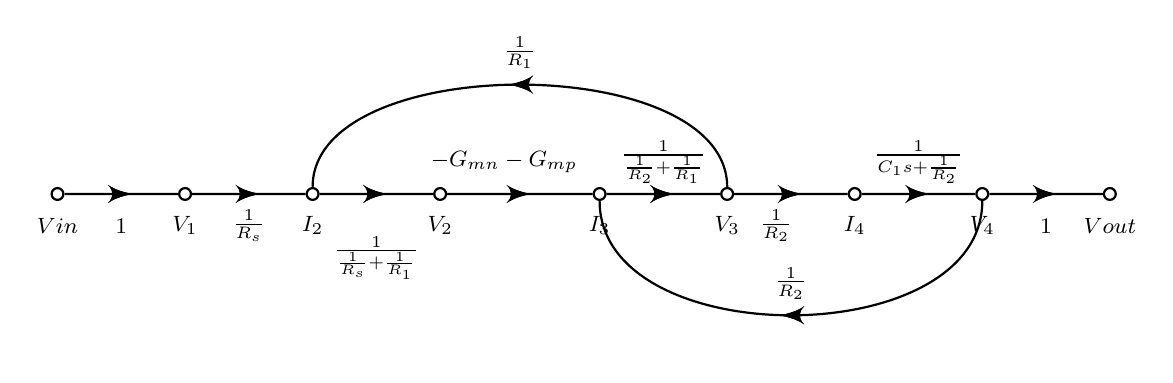
\begin{tikzpicture}[scale = 0.3,x=0.045cm,y=-0.045cm] % STYLES


%~~~~~~~~~~~~~~~~~~~~~~~~~~~~~~~~~~~~~~~~~~~~~~~~~~
% Set Nodes
%~~~~~~~~~~~~~~~~~~~~~~~~~~~~~~~~~~~~~~~~~~~~~~~~~~
\node[Node] (N1) at (173, 262) {};
\node[NodeName] at ($ (N1) + (0, 30) $) {$V_{1}$};

\node[Node] (N2) at (803, 262) {};
\node[NodeName] at ($ (N2) + (0, 30) $) {$I_{4}$};

\node[Node] (N3) at (53, 262) {};
\node[NodeName] at ($ (N3) + (0, 30) $) {$Vin$};

\node[Node] (N4) at (293, 262) {};
\node[NodeName] at ($ (N4) + (0, 30) $) {$I_{2}$};

\node[Node] (N5) at (923, 262) {};
\node[NodeName] at ($ (N5) + (0, 30) $) {$V_{4}$};

\node[Node] (N6) at (683, 262) {};
\node[NodeName] at ($ (N6) + (0, 30) $) {$V_{3}$};

\node[Node] (N7) at (1043, 262) {};
\node[NodeName] at ($ (N7) + (0, 30) $) {$Vout$};

\node[Node] (N8) at (413, 262) {};
\node[NodeName] at ($ (N8) + (0, 30) $) {$V_{2}$};

\node[Node] (N9) at (563, 262) {};
\node[NodeName] at ($ (N9) + (0, 30) $) {$I_{3}$};



%~~~~~~~~~~~~~~~~~~~~~~~~~~~~~~~~~~~~~~~~~~~~~~~~~~
% Set Branches
%~~~~~~~~~~~~~~~~~~~~~~~~~~~~~~~~~~~~~~~~~~~~~~~~~~
%Branch from Node N5 to Node N7
\draw [->-, Connection, MarkMiddle=1] (N5) ..controls(968.0, 262.0) and (998.0, 262.0) .. (N7);
\node[ArrowName] at($ (middle_1) + (0.0, 30.0) $) {$1$};

%Branch from Node N1 to Node N4
\draw [->-, Connection, MarkMiddle=2] (N1) ..controls(218.0, 262.0) and (248.0, 262.0) .. (N4);
\node[ArrowName] at($ (middle_2) + (0.0, 30.0) $) {$\frac{1}{R_{s}}$};

%Branch from Node N9 to Node N6
\draw [->-, Connection, MarkMiddle=3] (N9) ..controls(608.0, 262.0) and (638.0, 262.0) .. (N6);
\node[ArrowName] at($ (middle_3) + (0.0, -30.0) $) {$\frac{1}{\frac{1}{R_{2}} + \frac{1}{R_{1}}}$};

%Branch from Node N5 to Node N9
\draw [->-, Connection, MarkMiddle=4] (N5) ..controls(923.0, 412.0) and (563.0, 412.0) .. (N9);
\node[ArrowName] at($ (middle_4) + (0.0, -30.0) $) {$\frac{1}{R_{2}}$};

%Branch from Node N6 to Node N4
\draw [->-, Connection, MarkMiddle=5] (N6) ..controls(683.0, 127.0) and (293.0, 127.0) .. (N4);
\node[ArrowName] at($ (middle_5) + (0.0, -30.0) $) {$\frac{1}{R_{1}}$};

%Branch from Node N4 to Node N8
\draw [->-, Connection, MarkMiddle=6] (N4) ..controls(338.0, 262.0) and (368.0, 262.0) .. (N8);
\node[ArrowName] at($ (middle_6) + (0.0, 60.0) $) {$\frac{1}{\frac{1}{R_{s}} + \frac{1}{R_{1}}}$};

%Branch from Node N3 to Node N1
\draw [->-, Connection, MarkMiddle=7] (N3) ..controls(98.0, 262.0) and (128.0, 262.0) .. (N1);
\node[ArrowName] at($ (middle_7) + (0.0, 30.0) $) {$1$};

%Branch from Node N2 to Node N5
\draw [->-, Connection, MarkMiddle=8] (N2) ..controls(848.0, 262.0) and (878.0, 262.0) .. (N5);
\node[ArrowName] at($ (middle_8) + (0.0, -30.0) $) {$\frac{1}{C_{1} s + \frac{1}{R_{2}}}$};

%Branch from Node N6 to Node N2
\draw [->-, Connection, MarkMiddle=9] (N6) ..controls(728.0, 262.0) and (758.0, 262.0) .. (N2);
\node[ArrowName] at($ (middle_9) + (-14.0, 30.0) $) {$\frac{1}{R_{2}}$};

%Branch from Node N8 to Node N9
\draw [->-, Connection, MarkMiddle=10] (N8) ..controls(458.0, 262.0) and (518.0, 262.0) .. (N9);
\node[ArrowName] at($ (middle_10) + (-15.0, -30.0) $) {$- G_{mn} - G_{mp}$};



	\end{tikzpicture}
\end{document}